\documentclass{beamer}
\usetheme{Boadilla}

\title{Automated Negotiation}
\subtitle{Tournament based Negotiation}
\author{Group 1}
\date{}

\begin{document}
	\frame {
		\titlepage
	}
	\frame {
		\frametitle{Recap}
		
		\begin{block}{Automated Negotiation}
		Two agents take turns making offers until one accepts or the time runs out.
		
		Both agents have different preferences, an agent's preferences are unknown to the other agent.
		\end{block}
		
		\begin{block}{Outcome Space}
		There are one or more issues under negotiation.
		
		The possible values any issue can take can have different utilities for different opponents, and the weight of any issue can be different as well.
		\end{block}
	}
	\frame{
		\frametitle{The Genius Framework}
		\begin{block}{The Program}
		The Genius framework is a Java program allows you to define negotiation scenarios and preference profiles, and to let agents negotiate against each other.
		\end{block}
		
		\begin{block}{The Library}
		The Genius framework also comes with a library to implement your own agents in Java, which you can then add to the program.
		\end{block}
	}
	\frame{
		\frametitle{The Genius Framework}
		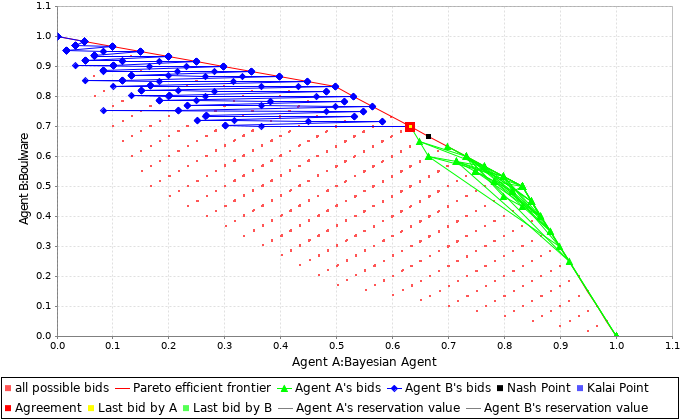
\includegraphics[scale=0.5]{example}
	}
	\frame{
		\frametitle{Our Project}
		\framesubtitle{Optimal Stopping}
		Our initial subject was 'Optimal Stopping'.

		\begin{block}{Optimal Stopping}
		Optimal Stopping focuses on the sub-problem of when to accept
		\end{block}

		\begin{block}{Problem 1}
		Turn-based
		% The original paper assumes you know how many turns are left. The agent is tested against agents which are not designed around this information and as such we don't want to use it. We estimate the remaining turns using knowledge about the time spent and remaining instead.
		\end{block}		
		
		\begin{block}{Problem 2}
		Modeling the opponent		
		% The behavior depends significantly on the model of your opponent.
		% We implemented one model which assumes the incoming utilities are uniform on the whole domain.
		%We implemented another model which assumes the incoming utilities are normally distributed, the mean and standard deviation are measured using incoming offers.
		\end{block}
	}
	\frame{
		\frametitle{Our Project}
		\framesubtitle{Bayesian Agent}
		\begin{block}{Motivation}
		% Our initial idea was to make this agent more interesting by adding bidding behavior, whereas the original agent just waits for offers until it accepts or time runs out.
		Build on optimal stopping by adding bidding behavior		
		\end{block}
		
		\begin{block}{Bayesian agent}
		Update beliefs about opponent's weights using the Bayesian rule under some assumptions:
		\begin{itemize}
		\item Conflict issues
		\item Offers represent true preferences
		\item Only use integer issues
		\end{itemize}
		Create counter-offers based on these beliefs
		% Explain how
		\end{block}
	}
	\frame{
		\frametitle{Our Project}
		\framesubtitle{SD Analyzer}
		\begin{block}{Idea}
		% Our initial idea was to make this agent more interesting by adding bidding behavior, whereas the original agent just waits for offers until it accepts or time runs out.	
		\end{block}
	}
	\frame{
		\frametitle{Our Project}
		\framesubtitle{Our Agents}
		\begin{block}{UniformAccepter}
		UniformAccepter uses optimal stopping, assuming the opponent makes uniform offers on the whole domain.
		\end{block}
		
		\begin{block}{NormalAccepter}
		NormalAccepter uses optimal stopping, assuming the opponent will make normally distributed offers like those observed so far.
		\end{block}
	}
	\frame{
		\frametitle{Our Project}
		\framesubtitle{Our Agents - part 2}
		\begin{block}{Bayesian}
		Bayesian uses preference estimation with target utility like Boulware.
		\end{block}
		
		\begin{block}{UniformBayesian and NormalBayesian}
		UniformBayesian and NormalBayesian are the same as Bayesian, except their target utilities are determined by the same algorithm that UniformAccepter and NormalAccepter respectively use.
		\end{block}
	}
	\frame{
		\frametitle{Our Project}
		\framesubtitle{Our Agents - part 3}
		\begin{block}{SDAnalyzer}
		Use variation instead of the actual value to estimate opponents preferences, with Boulwarez
		\end{block}
	}
	\frame{
		\frametitle{Demo}
	}
	
	\frame{
		\frametitle{Future works}
		\begin{itemize}
		\item Improved models of opponents preferences (e.g. GPR)
		\item Can optimal stopping benefit from making offers?
		\end{itemize}
		
	}
\end{document}